%&pdflatex
\subsection{Ottenere Debian 8 "jessie"}
Ogni versione Debian ha un \textit{nome in codice}: quello di Debian 8 è \textit{"jessie"}. Attualmente Debian 8 è l'ultima versione disponibile. Quando sarà rilasciata, Debian 9 si chiamerà \textit{"stretch"} --- al momento in \textit{testing}. In quanto segue tratteremo solo \textbf{Debian 8 "jessie"}: nel caso che Debian 9 (o una versione ancora più recente) sia stata rilasciata come \textit{stable}, il lettore è invitato a scaricare la nuova versione, tenendo però presente che quanto scritto in questo testo potrebbe non essere più interamente valido.

Debian 8 "jessie" è scaricabile dal sito:

\begin{graybox}
	\texttt{https://www.debian.org/distrib/}
\end{graybox}

Nella pagina dovrebbe trovarsi quanto mostrato in Figura \vref{fig:get-debian}.

\begin{figure}[ht]
	\centering
	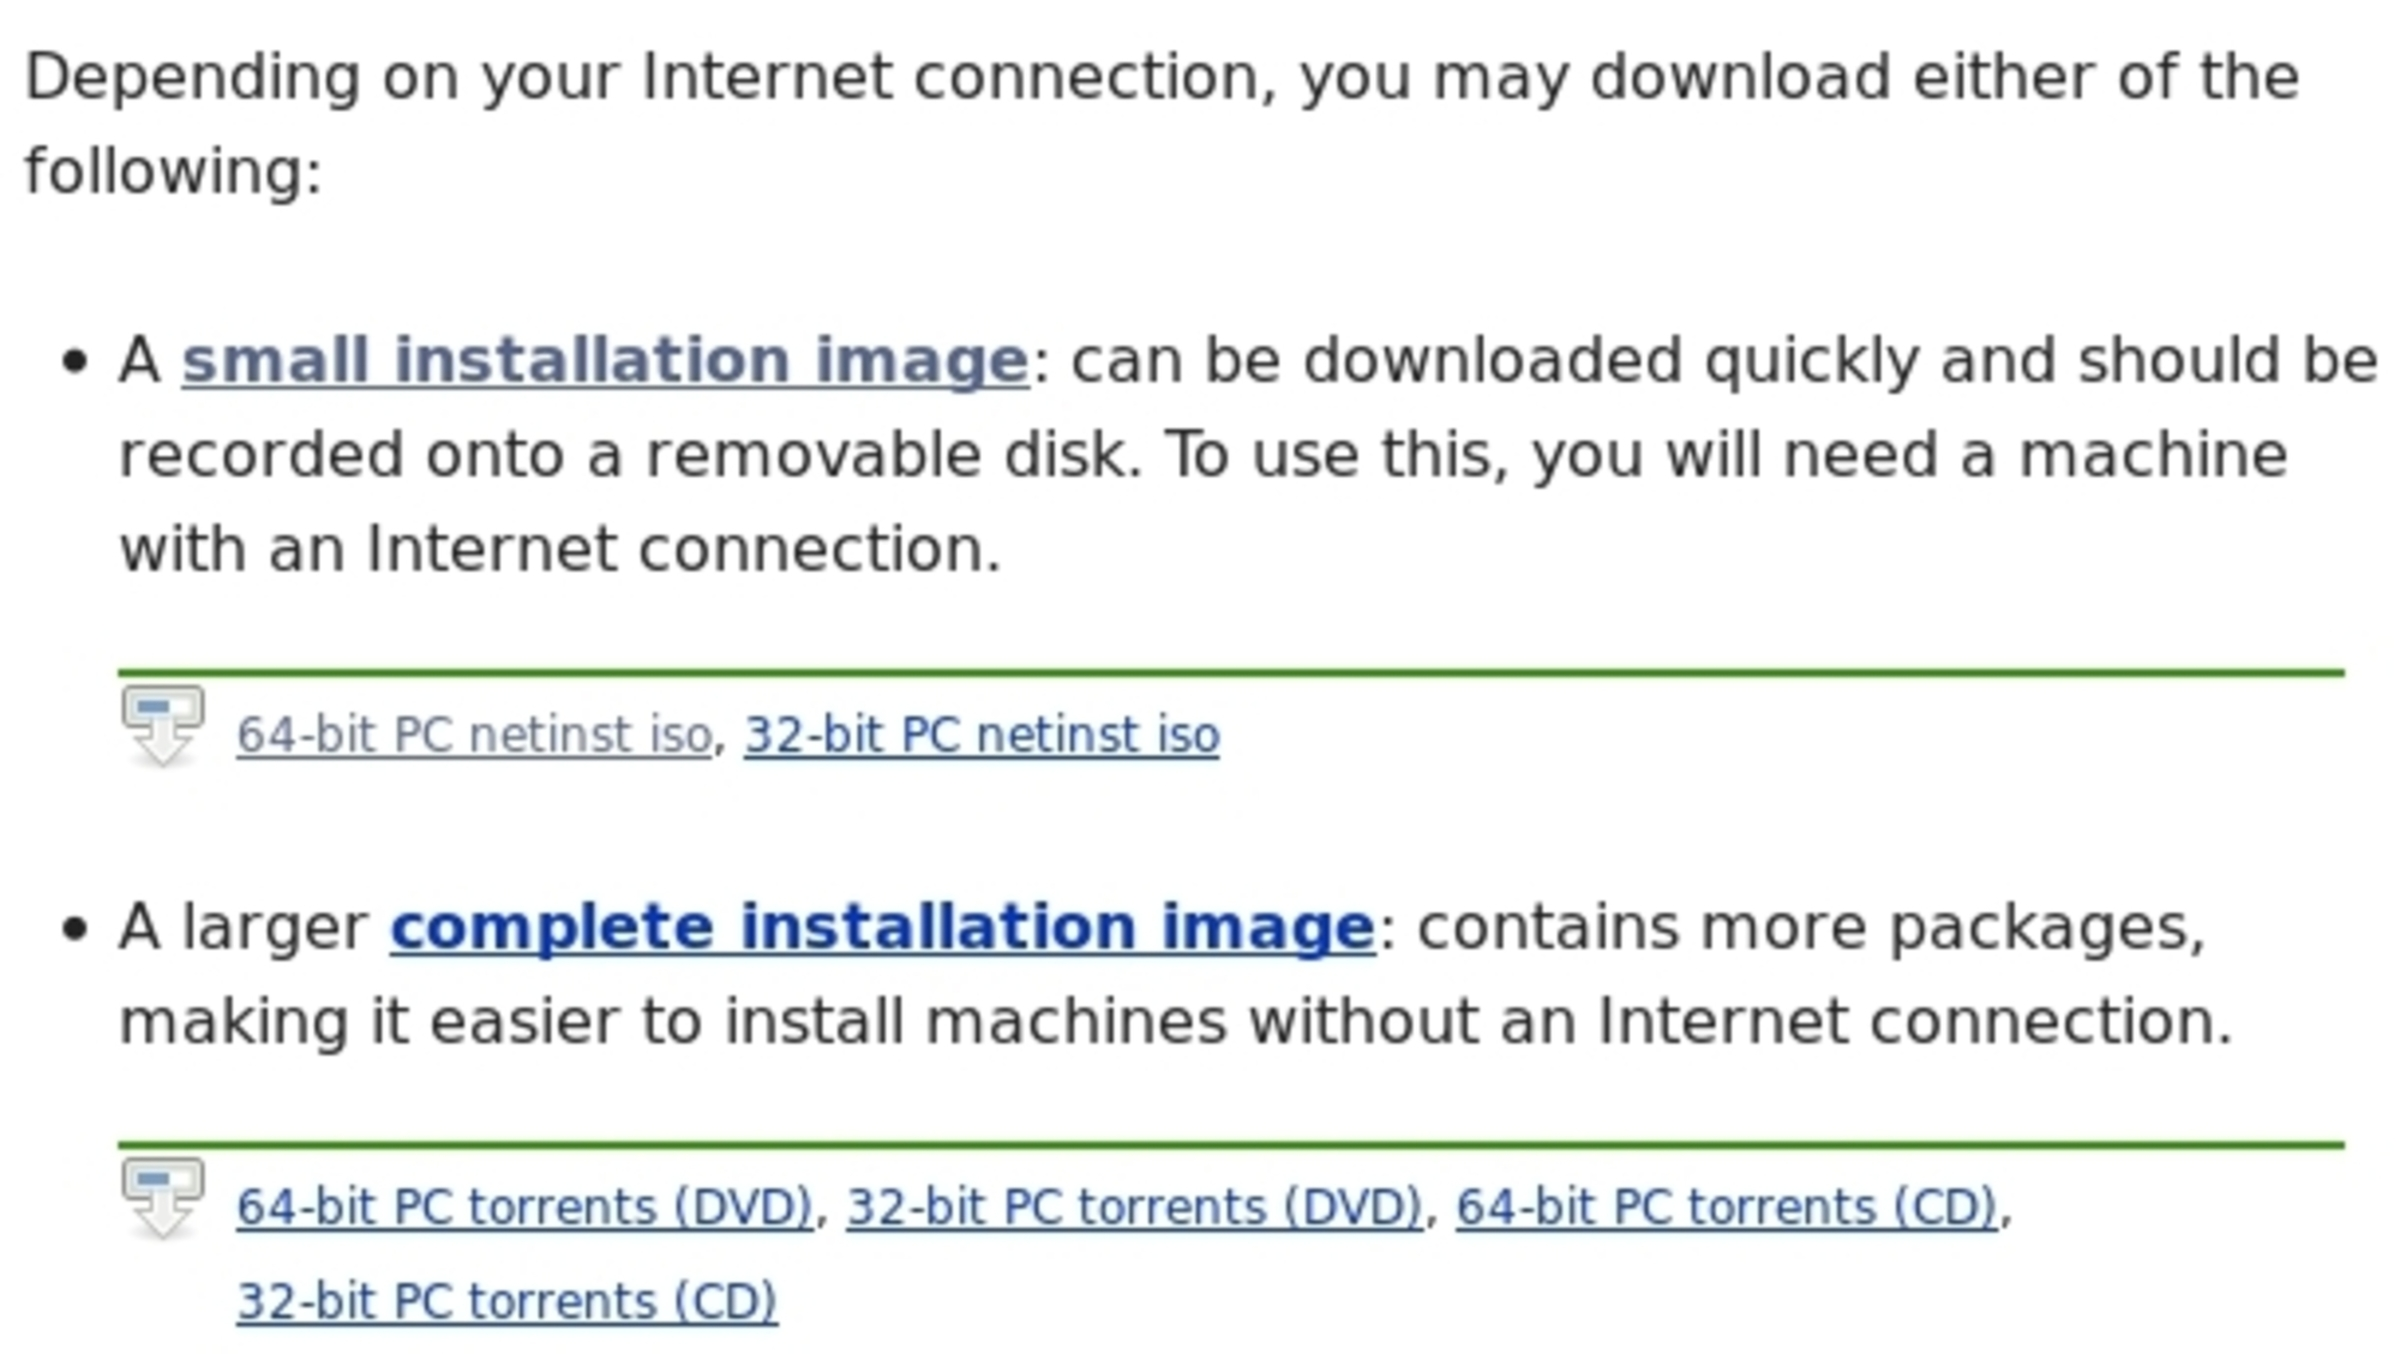
\includegraphics[resolution=600]{get-debian}
	\caption{Pagina di download di Debian}
	\label{fig:get-debian}
\end{figure}

Possiamo scegliere tra due tipi di file immagine: \textit{small (netinst)} e \textit{complete}. Non c'è alcuna differenza tra i due, se non per il fatto che il primo richiede una connessione a internet per l'installazione mentre il secondo no. Il consiglio è di utilizzare la netinst (small) in quanto richiede meno tempo per il download. Dobbiamo però anche scegliere tra due diverse versioni: \textit{64-bit PC amd64} (valida anche per architetture Intel, non inganni il nome) e \textit{32-bit PC i386}. I moderni computer hanno tutti architettura a 64 bit: l'architettura a 32 bit è obsoleta, ma in circolazione sono ancora presenti computer con questa architettura. Per determinare l'architettura del computer da Windows Vista/7 basta seguire alcuni semplici passi: \texttt{Menu Start} > \texttt{Sistema} > click destro su \texttt{Computer} > \texttt{Proprietà} e l'architettura comparirà in mezzo ad altre informazioni. Se il computer è stato acquistato con Windows 8 o successivi, allora sicuramente ha un'architettura a 64 bit; se invece è stato acquistato con Windows XP, allora sicuramente ha un'architettura a 32 bit.

\begin{graybox}
	\textbf{ATTENZIONE:} quanto detto sopra vale solo per computer con architetture Intel o AMD (le più diffuse). Debian però supporta anche altre architetture (ARM, PowerPC, MIPS, e altre ancora). Le immagini per queste architetture speciali, sono disponibili all'indirizzo:

	\texttt{https://www.debian.org/distrib/netinst}
\end{graybox}

Per poter seguire la procedura di installazione descritta nel Capitolo \vref{ch:install}, è necessario scaricare l'\textit{immagine ISO} sul proprio PC.
